\documentclass{article}
\usepackage[superscript,biblabel]{cite}
\usepackage{graphicx}
\usepackage{float}
\usepackage{multirow}

\graphicspath{{../../analysis/images/}}
\bibliographystyle{naturemag}

\title{Epistasis is widespread in the genetic control of transcription in humans}
\date{}
\author{Gibran Hemani, Konstantin Shakhbazov, Joseph E Powell}

\begin{document}

\maketitle


\begin{abstract}
A long standing question in evolution and human genetics is the extent to which epistasis, the phenomenon whereby one polymorphism's effect on a trait depends on other polymorphisms present in the genome, contributes to complex traits \cite{Carlborg2004, Hill2008a, Crow2010}. Though epistasis has been demonstrated in artificial gene manipulation studies in model organisms \cite{Costanzo2010, Bloom2013}, and some examples have been shown in other species \cite{Carlborg2006}, few convincing examples exist for epistasis amongst natural polymorphisms in human traits \cite{Strange2010, Evans2011}. Its absence from empirical findings may simply be due to its unimportance in the genetic control of complex traits \cite{Hill2008a, Crow2010}, but we sought to test the hypothesis that it has previously been too technically difficult to detect due to statistical power and computational issues \cite{Cordell2009}. Here we show that, using advanced computation techniques \cite{Hemani2011} and a gene expression study design, evidence for multiple instances of epistasis is found. In a cohort of 846 individuals with data on 7339 gene expression levels in whole blood, we found that after stringent correction for multiple testing there were 501 significant pairwise epistatic interactions acting on the expression levels of 238 genes. Thirty interactions replicated in two independent datasets \cite{Metspalu2004, Fehrmann2011} following Bonferroni correction for multiple testing. Of the SNPs that did not pass this replication threshold, there was significant enrichment for interaction effects (316 of 434 above the 2.5\% confidence interval for uniformly distributed $p$-values, $p < 1.0 \times 10^{-16}$). We provide evidence of functional enrichment for the interacting SNPs, for instance 44 of the genetic interactions are located within 5Mb of regions of known intra-cellular chromosome interactions \cite{Lieberman-Aiden2009} ($p < 1.8 \times 10^{-10}$). Multi-locus epistatic interactions control 129 genes, whereby one \emph{cis}-acting single nucleotide polymorphism (SNP) is modulated by several trans-acting SNPs. For example MBNL1 is controlled by an additive effect at rs13069559 which itself is controlled by \emph{trans}-SNPs on 14 different chromosomes, with nearly identical genotype-phenotype (GP) maps for each \emph{cis}-\emph{trans} interaction. This study presents the first strong evidence for multiple instances of epistatic genetic effects emerging from natural genetic variation in humans, and demonstrates its significant contribution to the variance of gene expression.
\end{abstract}


\section{Main text}

% \subsection{Introduction}
The past decade has seen a tremendous amount of activity in mapping genetic polymorphisms that underlie complex traits. Typically, SNPs are treated using an additive model where they are assumed to contribute linearly, independently, and cumulatively to the mean of a trait. This has been successful in identifying thousands of associations \cite{Visscher2012}, but to date there is little empirical exploration of the role that epistasis plays in the architecture of complex traits in humans \cite{Strange2010, Evans2011}, though its contribution to phenotypic variance is frequently the subject of debate \cite{Carlborg2004, Hill2008a, Crow2010}. Outside the prism of human association studies there is widespread evidence for epistasis, not only at the molecular scale from artificially induced mutations \cite{Costanzo2010} but also at the evolutionary scale in fitness adaptation \cite{Weinreich2006} and speciation \cite{Breen2012}. Here we demonstrate that amongst common polymorphisms multiple instances of statistical epistasis can be detected in human traits, and that some quantification of its relative contribution to phenotypic variance can be made.

Detection of epistasis is hampered by power issues for several reasons, including increased dependence on linkage disequilibrium (LD) between causal SNPs and observed SNPs \cite{Weir2008, Hemani2013}, increased model complexity in fitting interaction terms \cite{Marchini2005}, and more extreme significance thresholds to account for increased multiple testing \cite{Cordell2009}. When genetic effect sizes are small, as is expected in most complex traits of interest \cite{Visscher2012}, the power to detect epistasis diminishes rapidly. There are two simple ways to overcome this problem. One is by using extremely large sample sizes \cite{LangoAllen2010}; another is by analysing traits that are likely to have large effect sizes. Because our focus was to ascertain the extent to which epistasis exists amongst natural genetic variation we designed a study around the latter approach and searched for epistatic genetic effects that influence gene expression levels. Transcription levels can be measured for thousands of genes. These traits are largely heritable but on average less polygenic than high level phenotypes \cite{Powell2013}, thus it is expected that many genetic effects will be relatively large, maximising the chance at detecting epistasis, should it exist.


% \subsection{Initial search in discovery set and replication}
In our discovery dataset (Brisbane Systems Genetics Study, BSGS \cite{Powell2012}) of 846 individuals genotyped at 528509 SNPs, we exhaustively tested every pair of SNPs for genetic interactions against each of 7339 expression traits in whole blood. After stringent filtering and multiple testing correction we had identified 501 putative genetic interactions influencing 238 gene expression levels. Of the 501 discovery interactions, 434 had available data and passed filtering (Methods) in two independent replication datasets, Fehrmann \cite{Fehrmann2011} and the Estonian Genomics Centre University of Tartu (EGCUT) \cite{Metspalu2004}, in which we saw convincing evidence for replication. We used the summary statistics from the replication datasets to perform a meta analysis to obtain an independent $p$-value for the putative interactions, and 30 were significant after applying a Bonferroni correction for multiple testing (Table \ref{tab:bonferroni}). These significant interactions exhibited remarkable similarity in GP maps between all three datasets (Figure \ref{fig:gpmaps}).

Additionally, there was extreme enrichment for interaction effects among the discovery SNPs that did not reach the stringent significance threshold for replication (Figure \ref{fig:qqMeta}). We observed that 316 of the remaining 404 discovery SNPs had replication interaction $p$-values exceeding the one-tailed 2.5\% confidence interval under the null distribution of no effects ($p << 1.0 \times 10^{-16}$, Supplementary Figure \ref{fig:qqMetaNonsig}). The congruence of the epistatic networks in discovery and replication datasets is shown in Figure \ref{fig:fireworks}, demonstrating that these complex genetic patterns are common even across independent populations. A further replication was attempted using the Centre for Health Discovery and Wellbeing (CHDWB) dataset \cite{Preininger2013}, but only 185 of the SNP pairs passed filtering because the sample size was small ($n=139$), and due to insufficient power we found no evidence for replication. It should be noted that although it is a necessary step to establish the veracity of the signals from the discovery set, replication of epistasis is theoretically difficult because the dependence on LD between observed SNPs and causal variants is on average three orders of magnitude higher than it is for independent additive effects \cite{Weir2008, Hemani2013}. Therefore these results are very encouraging with regards to the detection and replication of epistasis.


% \subsection{Patterns of epistasis}
Though seldom the focus of association studies, SNPs with known main effects are often tested for additive $\times$ additive genetic interactions \cite{Cordell2009}, but our analysis shows that this is unlikely to be the most effective strategy for its detection. The majority of our discovery interactions comprised of one SNP that had a previously known association and one SNP that had no previous association in the dataset \cite{Powell2013} (439 out of 501). Only 9 interactions were between SNPs that both had marginal effects while 64 were between SNPs that had no known marginal effects. Additionally, we observed that the largest epistatic variance component for the 501 interactions were divided amongst additive $\times$ additive, additive $\times$ dominance and dominance $\times$ dominance terms proportional to what is expected by chance ($p = 0.22$ for divergence from expectation). This is not surprising because the patterns of epistasis used for statistical decomposition are not designed to resemble biological function \cite{Cockerham1954}.

We observed a wide range of significant GP maps (Figure \ref{fig:gpmaps}) but the most common pattern of epistasis that we detected involved a \emph{trans}-SNP masking the effect of an additive \emph{cis}-SNP. For example, MBNL1 (involved in RNA modification and regulation of splicing \cite{Ho2004}) has a \emph{cis} effect at rs13069559 which in turn is controlled by 13 \emph{trans}-SNPs and one \emph{cis}-SNP that each exhibit a masking pattern, such that when the \emph{trans}-SNP is homozygous for the masking allele the decreasing allele of the \emph{cis}-SNP no longer has an affect. We observed that nine of the 14 masking SNPs are located in intronic regions (proportion of SNP panel in introns $= 0.05$, $p = 3.11 \times 10^{-9}$), and each of these interactions have evidence for replication in at least one dataset and six are significant at the Bonferroni level (Supplementary Figure \ref{fig:circleplots}).


% \subsection{Functional annotation}
Of the discovery interactions, 47 were \emph{cis}-\emph{cis} acting (both SNPs were on the same chromosome as the expression gene), 441 were \emph{cis}-\emph{trans}-acting, and 13 were \emph{trans}-\emph{trans}-acting. In total the 501 interactions comprised 781 unique SNPs, which we analysed for functional enrichment. We tested the SNPs for cell-type specific overlap with transcriptionally active chromatin regions, tagged by histone-3-lysine-4,3-methylation (H3K4me3) chromatin marks, in 34 cell types \cite{Trynka2013}. There was significant enrichment for \emph{cis}-acting SNPs in haematopoeitic cell types only ($p < 1 \times 10^{-4}$ for the three tissues with the strongest enrichment are significant at after adjusting for multiple testing, Supplementary Figure \ref{fig:transh3k4me3}). However \emph{trans}-acting SNPs did not show any tissue specific enrichment ($p > 0.1$ for all tissues, Supplementary Figure \ref{fig:transh3k4me3}). 
This difference between \emph{cis} and \emph{trans} SNPs suggests that there is a range of molecular mechanisms by which epistasis might arise and the cis-SNPs may provide tissue specificity in these interactions. There is also strong enrichment for SNPs to be localised in enhancer regions \cite{Ward2012a} (Supplementary Figure \ref{fig:enhancers}). This enrichment is consistent for both \emph{cis} and \emph{trans} SNPs ($p < 1 \times 10^{-6}$). In particular, there was substantial enrichment for the GATA2 binding motif within 1kb of all epistatic SNPs, a known regulator of transcription in haematopoietic cells \cite{Tsai1994} ($p = 1 \times 10^{-40}$).

We also demonstrate a putative novel mechanism by which biological function can lead to epistatic genetic variance. It has been shown that chromosomal regions spatially colocalise in the cell through chromatin interactions \cite{Lieberman-Aiden2009}. We cross referenced our epistatic SNPs with a map of chromosome interacting regions ($n = 96139$) in K562 blood cell lines \cite{Lan2012} and found that fifty epistatic interactions mapped to within 2Mb ($p < 1.8 \times 10^{-10}$), (Supplementary Figure \ref{fig:chromosomeinteractions}), but decyphering the exact cellular processes underlying this interaction requires further research.


% \subsection{Contribution of epistatic variance}
Though we present many instances of epistasis, quantifying its relative importance to complex traits in humans remains an open question. In this study we are able to identify 238 gene expression traits with at least one significant interaction given our experiment-wide threshold. How does this compare to the number of traits controlled by additive effects? The BSGS dataset has been previously analysed for additive effects at all expression traits \cite{Powell2012}, and if we take all the additive eQTLs that were significant at the epistatic threshold of $p < 2.91 \times 10^{-16}$ we find that 453 gene expression levels out of the 7339 analysed had at least one significant expression quantitative trait locus (eQTL). Therefore it can be argued that the number of instances of detectable epistasis are substantial.

However in terms of their contribution to complex traits a more important metric might be the proportion of the variance that the epistatic loci explain \cite{Hill2008a}. Ideally one would approach this question from a whole genome level \cite{Visscher2008} but this is intractable for non-additive variance components. Yet some inference can be made from the ascertained effects in these analyses and it is evident that additive variance is overall a larger component than epistatic variance, as has been argued previously \cite{Hill2008a, Crow2010}. Taking the additive effects detected in Powell \emph{et al} (2012) at the $p < 2.91 \times 10^{-16}$ threshold, we calculate that in total they explain 1.73\% of the total phenotypic variance of all 7339 probes. By contrast, the epistatic signals detected in this study explain 0.25\% of all phenotypic variance, approximately seven times lower than the additive variance. This is broadly in line with theory \cite{Hill2008a}, but there are two caveats to this comparison. Firstly the power of a 1 \emph{d.f.} test exceeds that of an 8 \emph{d.f.} test. Secondly the non-additive variance at causal variants is expected to be underestimated by observed SNPs in comparison to estimates for additive variance, due to differences in the rate of decay of the estimate of the genetic variance of the causal SNPs as LD decreases with the observed SNPs. Therefore this is likely to be a lower bound on the estimate of the relative contribution of epistasis to the genetic variance of gene expression.


% \subsection{Discussion}
Overall, we have demonstrated that it is possible to identify and replicate epistasis in complex traits amongst common human variants. The functional analysis of the significant epistatic loci suggests that there are a large number of possible mechanisms that can lead to non-additive genetic variation, thus it is not surprising that multiple instances of epistasis should be discovered in spite of statistical power limitations. Further research into such genetic effects may provide a useful portal to understanding molecular mechanisms with greater clarity. With data and computational techniques now widely available the search for epistasis in larger datasets for traits of broader interest is warranted.


\subsection{Methods Summary}
We searched for pairwise epistasis exhaustively in the BSGS discovery dataset \cite{Powell2012}, which comprises 846 individuals who are genotyped at 528509 autosomal SNPs and who have gene expression levels measured in whole blood samples for 7339 probes representing 6158 RefSeq genes. Recent hardware and software \cite{Hemani2011} advances made it possible to perform the $1.03 \times 10^{15}$ statistical tests to complete this analysis. We used permutation analysis \cite{Churchill1994a} to calculate an experiment-wide significance threshold of $2.91 \times 10^{-16}$ at the 5\% family-wise error rate (FWER). SNP pairs were modelled for full genetic effects, including marginal additive and dominance at both SNPs plus four interaction terms. Though we could have used a less complex model to improve statistical efficiency, we deemed it important to be agnostic about the type of epistasis that might exist, and therefore chose not to over-parameterise the test \cite{Marchini2005, Hemani2013}. Because there are many large marginal effects present in these data it was necessary to perform several filtering steps to exclude SNP pairs that were significant due to marginal effects alone. All SNP pairs with LD $r^2 > 0.1$ were removed, and were required to have at least five data points in all nine genotype classes. If multiple SNP pairs were present on the same chromosomes for a particular expression trait then only the sentinal SNP pair was retained. Finally, a nested test contrasting the full genetic model against the marginal additive and dominance model was performed for each remaining SNP pair (Methods), resulting in 501 significant interactions after Bonferroni correction for multiple testing of the filtered SNPs. The significant SNP pairs were carried forward for replication in two independent datasets that used the same expression assays for analysing transcription in whole blood, the Fehrmann dataset \cite{Fehrmann2011} ($n=1240$) and the Estonian Genome Centre University of the University of Tartu (EGCUT) dataset \cite{Metspalu2004} ($n=891$). Of these, 434 passed filtering in both replication datasets.


\clearpage
\section{Tables}

\begin{table}[ht]
\centering
\begin{tabular}{rlllrr}
  \hline
 & & & & \multicolumn{2}{c}{$-\log_{10} p$} \\
 & Gene (chr.) & SNP 1 (chr.) & SNP 2 (chr.) & Discovery & Replication \\
  \hline
1 & ADK (10)  & rs2395095 (10)  & rs10824092 (10)  & 6.69 & 39.82 \\
  2 & ATP13A1 (19)  & rs4284750 (19)  & rs873870 (19)  & 5.30 & 14.23 \\
  3 & C21ORF57 (21)  & rs9978658 (21)  & rs11701361 (21)  & 9.42 & 21.67 \\
  4 & CSTB (21)  & rs9979356 (21)  & rs3761385 (21)  & 11.99 & 42.27 \\
  5 & CTSC (11)  & rs7930237 (11)  & rs556895 (11)  & 7.16 & 33.53 \\
  6 & FN3KRP (17)  & rs898095 (17)  & rs9892064 (17)  & 16.16 & 59.95 \\
  7 & GAA (17)  & rs11150847 (17)  & rs12602462 (17)  & 13.91 & 32.60 \\
  8 & HNRPH1 (5)  & rs6894268 (5)  & rs4700810 (5)  & 15.38 & 10.37 \\
  9 & LAX1 (1)  & rs1891432 (1)  & rs10900520 (1)  & 19.16 & 29.24 \\
  10 & MBNL1 (3)  & rs16864367 (3)  & rs13079208 (3)  & 13.49 & 41.56 \\
  11 & MBNL1 (3)  & rs7710738 (5)  & rs13069559 (3)  & 7.92 & 9.28 \\
  12 & MBNL1 (3)  & rs2030926 (6)  & rs13069559 (3)  & 7.10 & 5.53 \\
  13 & MBNL1 (3)  & rs2614467 (14)  & rs13069559 (3)  & 5.74 & 5.30 \\
  14 & MBNL1 (3)  & rs218671 (17)  & rs13069559 (3)  & 7.63 & 5.23 \\
  15 & MBNL1 (3)  & rs11981513 (7)  & rs13069559 (3)  & 7.71 & 4.58 \\
  16 & MBP (18)  & rs8092433 (18)  & rs4890876 (18)  & 5.40 & 28.73 \\
  17 & NAPRT1 (8)  & rs2123758 (8)  & rs3889129 (8)  & 8.45 & 30.77 \\
  18 & NCL (2)  & rs7563453 (2)  & rs4973397 (2)  & 7.31 & 12.70 \\
  19 & PRMT2 (21)  & rs2839372 (21)  & rs11701058 (21)  & 4.81 & 4.06 \\
  20 & RPL13 (16)  & rs352935 (16)  & rs2965817 (16)  & 4.98 & 17.24 \\
  21 & SNORD14A (11)  & rs2634462 (11)  & rs6486334 (11)  & 7.31 & 23.22 \\
  22 & TMEM149 (19)  & rs807491 (19)  & rs7254601 (19)  & 12.16 & 145.78 \\
  23 & TMEM149 (19)  & rs8106959 (19)  & rs6926382 (6)  & 5.80 & 10.72 \\
  24 & TMEM149 (19)  & rs8106959 (19)  & rs914940 (1)  & 6.22 & 9.20 \\
  25 & TMEM149 (19)  & rs8106959 (19)  & rs2351458 (4)  & 7.30 & 8.00 \\
  26 & TMEM149 (19)  & rs8106959 (19)  & rs6718480 (2)  & 8.55 & 7.36 \\
  27 & TMEM149 (19)  & rs8106959 (19)  & rs1843357 (8)  & 6.21 & 6.00 \\
  28 & TMEM149 (19)  & rs8106959 (19)  & rs9509428 (13)  & 9.44 & 4.47 \\
  29 & TRA2A (7)  & rs7776572 (7)  & rs11770192 (7)  & 8.23 & 4.09 \\
  30 & VASP (19)  & rs1264226 (19)  & rs2276470 (19)  & 5.09 & 4.95 \\
   \hline
\end{tabular}
\caption{Epistatic interactions significant at the Bonferroni level in two replication sets. All $p$-values are for 4 \emph{d.f.} interaction tests (exact in Discovery and meta analysis for Replication).}
\label{tab:bonferroni}
\end{table}


\clearpage
\section{Figures}

\begin{figure}[H]
	\centering
	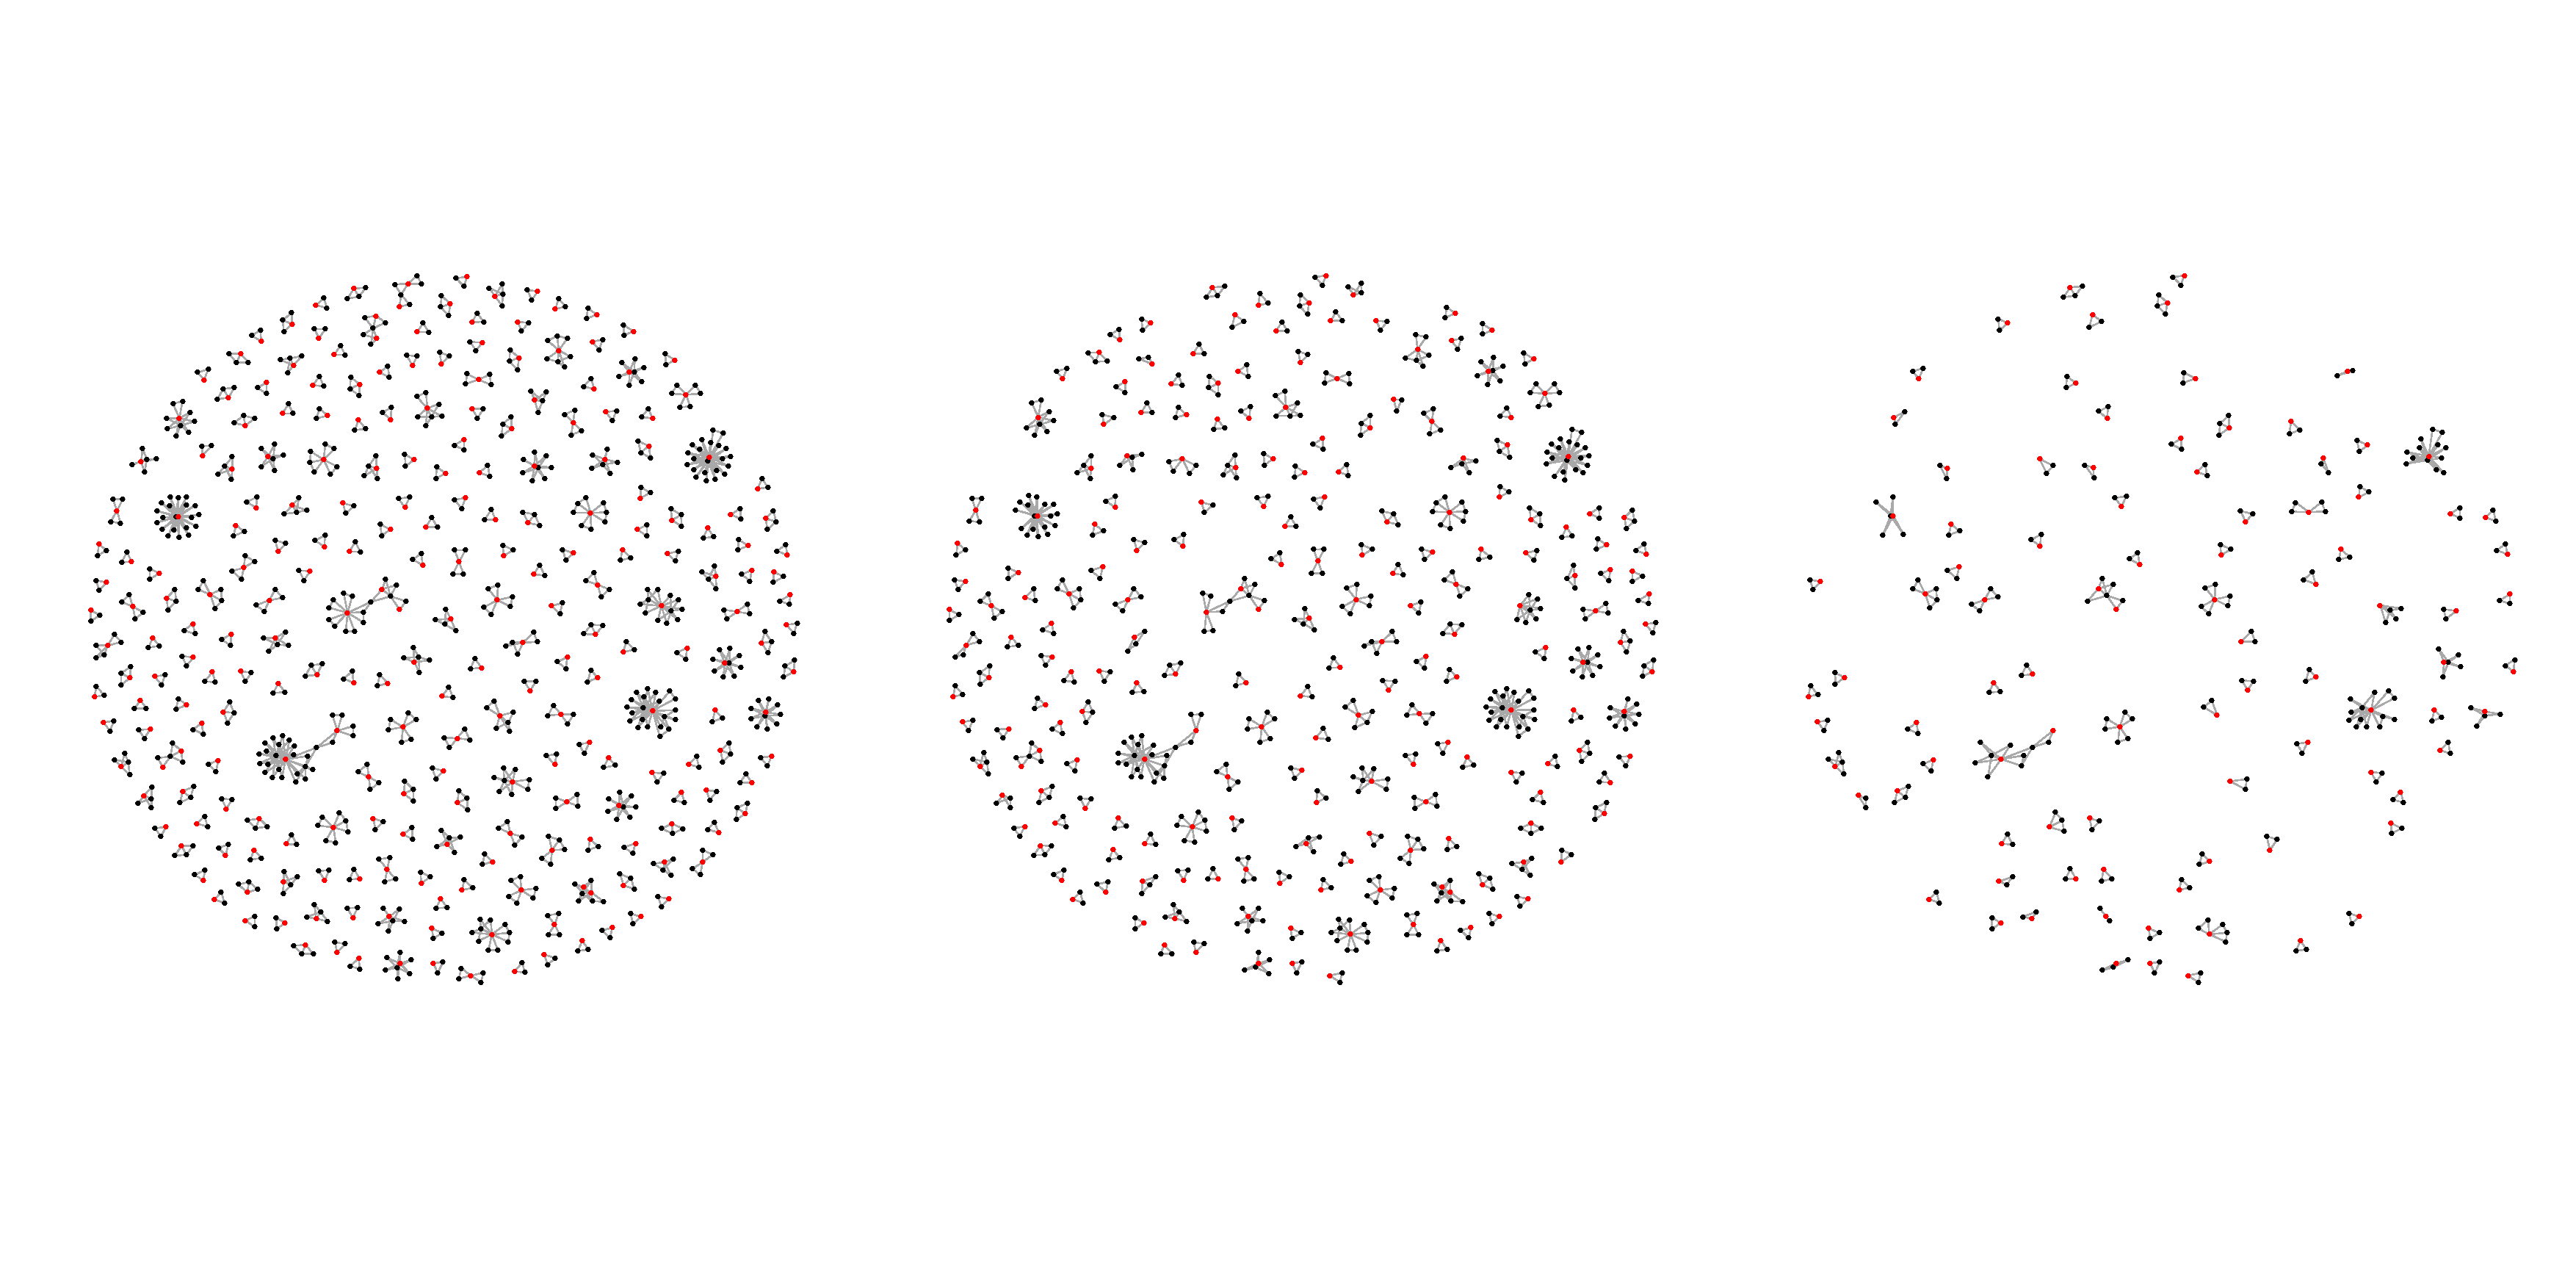
\includegraphics[width=5in]{graph_of_interactions.pdf}
	\caption{\textbf{Replication of epistatic networks in two cohorts} Panel A represents all 434 genetic interactions (edges) discovered in the discovery set. Panel B shows those interactions that were present at the 5\% FDR level in at least one replication dataset, and panel C shows which interactions were significant in both replication datasets. Red nodes represent probes and black nodes represent SNPs. The congruence between datasets is indicitive of the consistent epistatic instances in independent populations.}
	\label{fig:fireworks}
\end{figure}
\clearpage

\begin{figure}[H]
	\centering
	\includegraphics[width=2.5in]{gpbonfrep.pdf}
	\caption{\textbf{Replication of genotype-phenotype (GP) maps in two independent populations} The GP maps for each epistatic interaction that is significant at the Bonferroni level in both replication datasets are shown. Each GP map consists of nine tiles where each tile represents the expression level for that two-locus genotype class. Phenotypes are for gene transcript levels (dark coloured tiles = low expression, light coloured tiles = high expression). Columns of GP maps are for each independent population. Rows of GP maps are for each of 30 significantly replicated interactions, corresponding to the rows in Table \ref{tab:bonferroni}. There is a general trend of the GP maps replicating across all three datasets.}
	\label{fig:gpmaps}
\end{figure}
\clearpage

\begin{figure}[H]
	\centering
	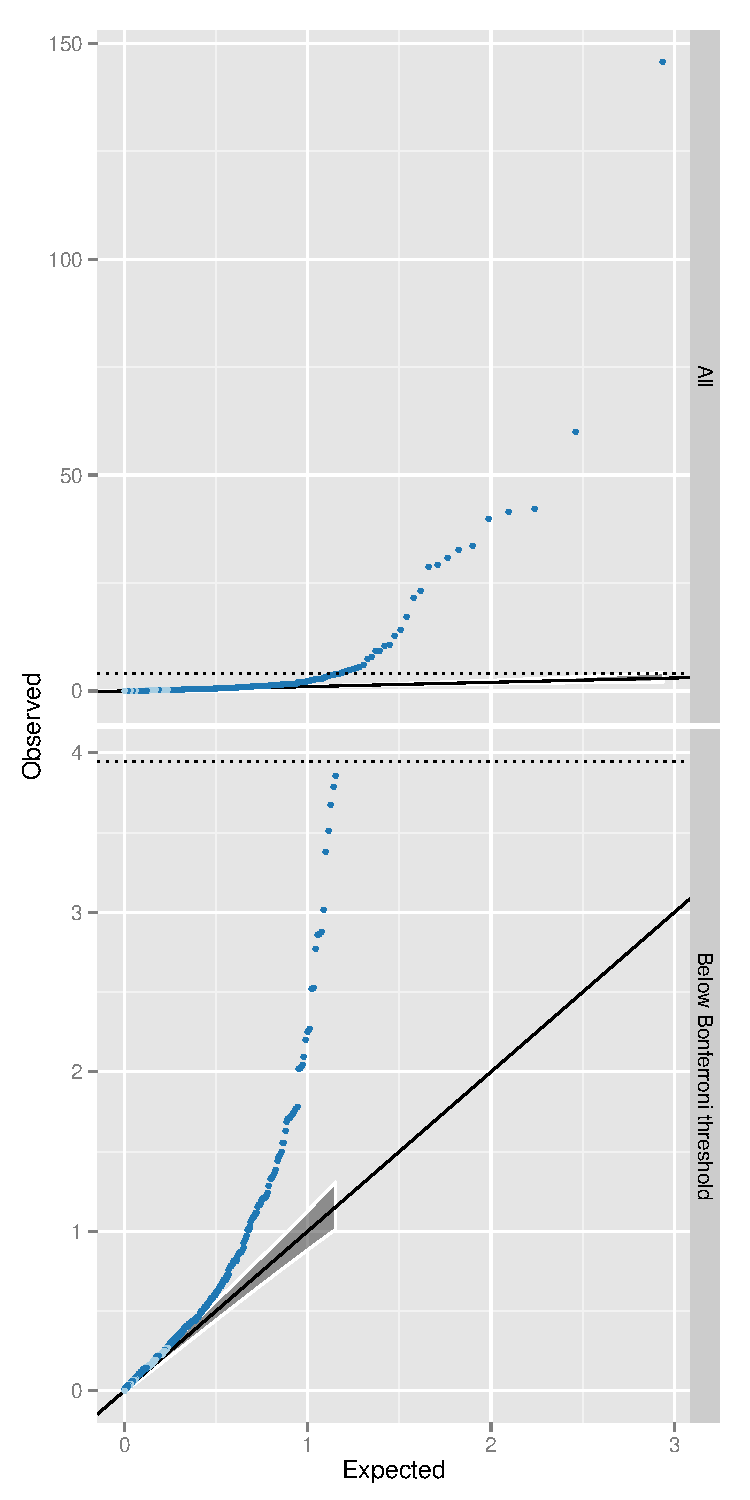
\includegraphics[width=2.5in]{qqMeta.pdf}
	\caption{\textbf{Q-Q plots of interaction $p$-values from replication datasets} Top panel shows all 434 discovery SNPs that were tested for interactions. Observed $p$-values ($y$-axis, $-\log_{10}$ scale) are plotted against the expected $p$-values ($x$-axis, $-\log_{10}$ scale). The multiple testing correction threshold for significance is denoted by a dotted line. Bottom panel shows the same data as the top panel but excluding the 30 interactions that were significant at the Bonferroni level in the replication datasets. The shaded grey area represents the 5\% confidence interval for the expected distribution of $p$-values. Dark blue points represent $p$-values that exceed the confidence interval, light blue are within the confidence interval.}
	\label{fig:qqMeta}
\end{figure}
\clearpage


\clearpage
\section{Supplementary Figures}
\setcounter{figure}{0}
\makeatletter 
\renewcommand{\thefigure}{S\@arabic\c@figure} 
\makeatletter 


\begin{figure}[H]
	\centering
	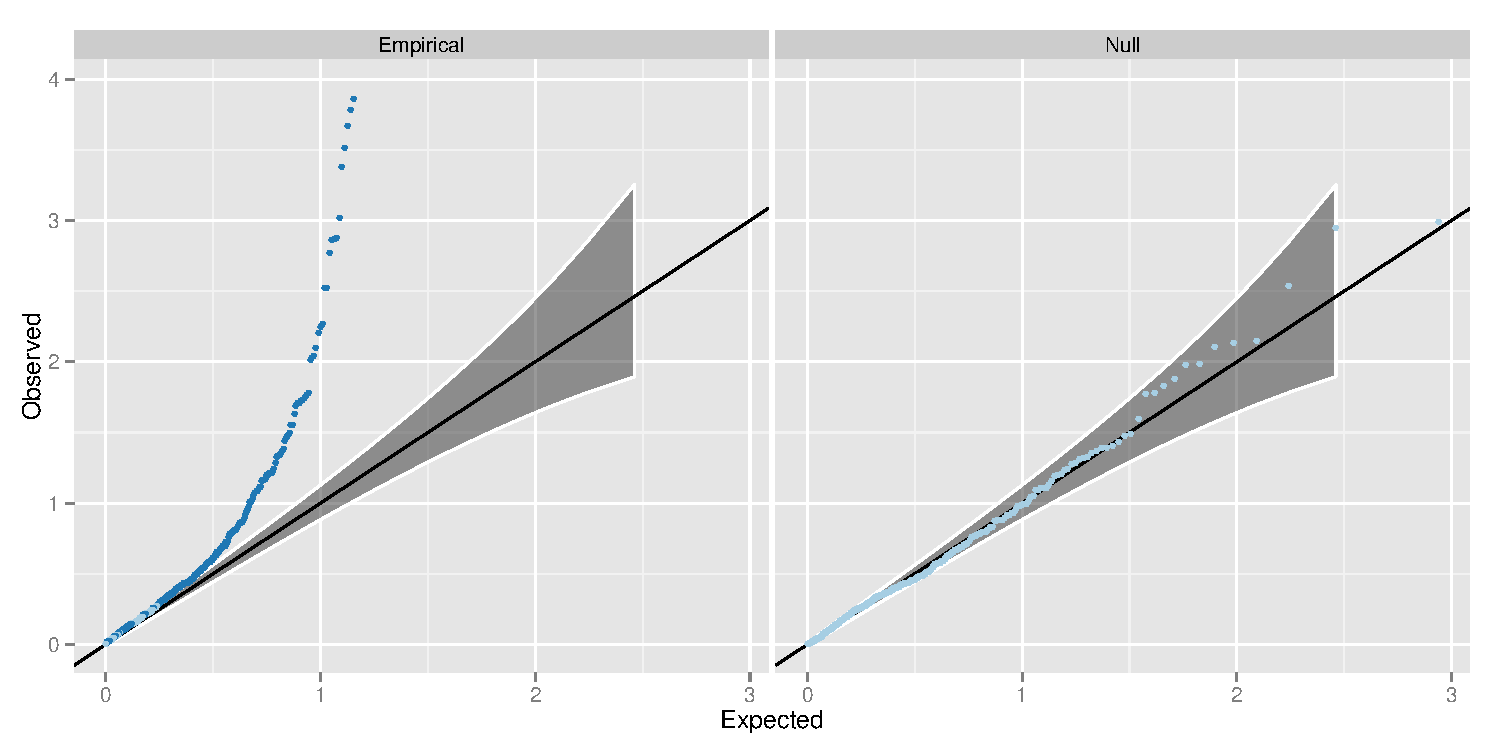
\includegraphics[width=5in]{qqMetaNonsig}
	\caption{\textbf{Q-Q plots of interaction $p$-values from replication datasets, excluding the 30 points significant at the Bonferroni level} The right panel (Null) shows the interaction $p$-values from a meta analysis across two independent datasets on 434 randomly drawn SNP pairs. The left panel (Empirical) shows the interaction $p$-values from the 404 putative interactions that were not significant at the Bonferroni correction threshold. Dark blue points represent $p$-values that surpass the 5\% FDR level, as in Figure \ref{fig:qqMeta}.}
\label{fig:qqMetaNonsig}
\end{figure}
\clearpage

\begin{figure}
	\centering
	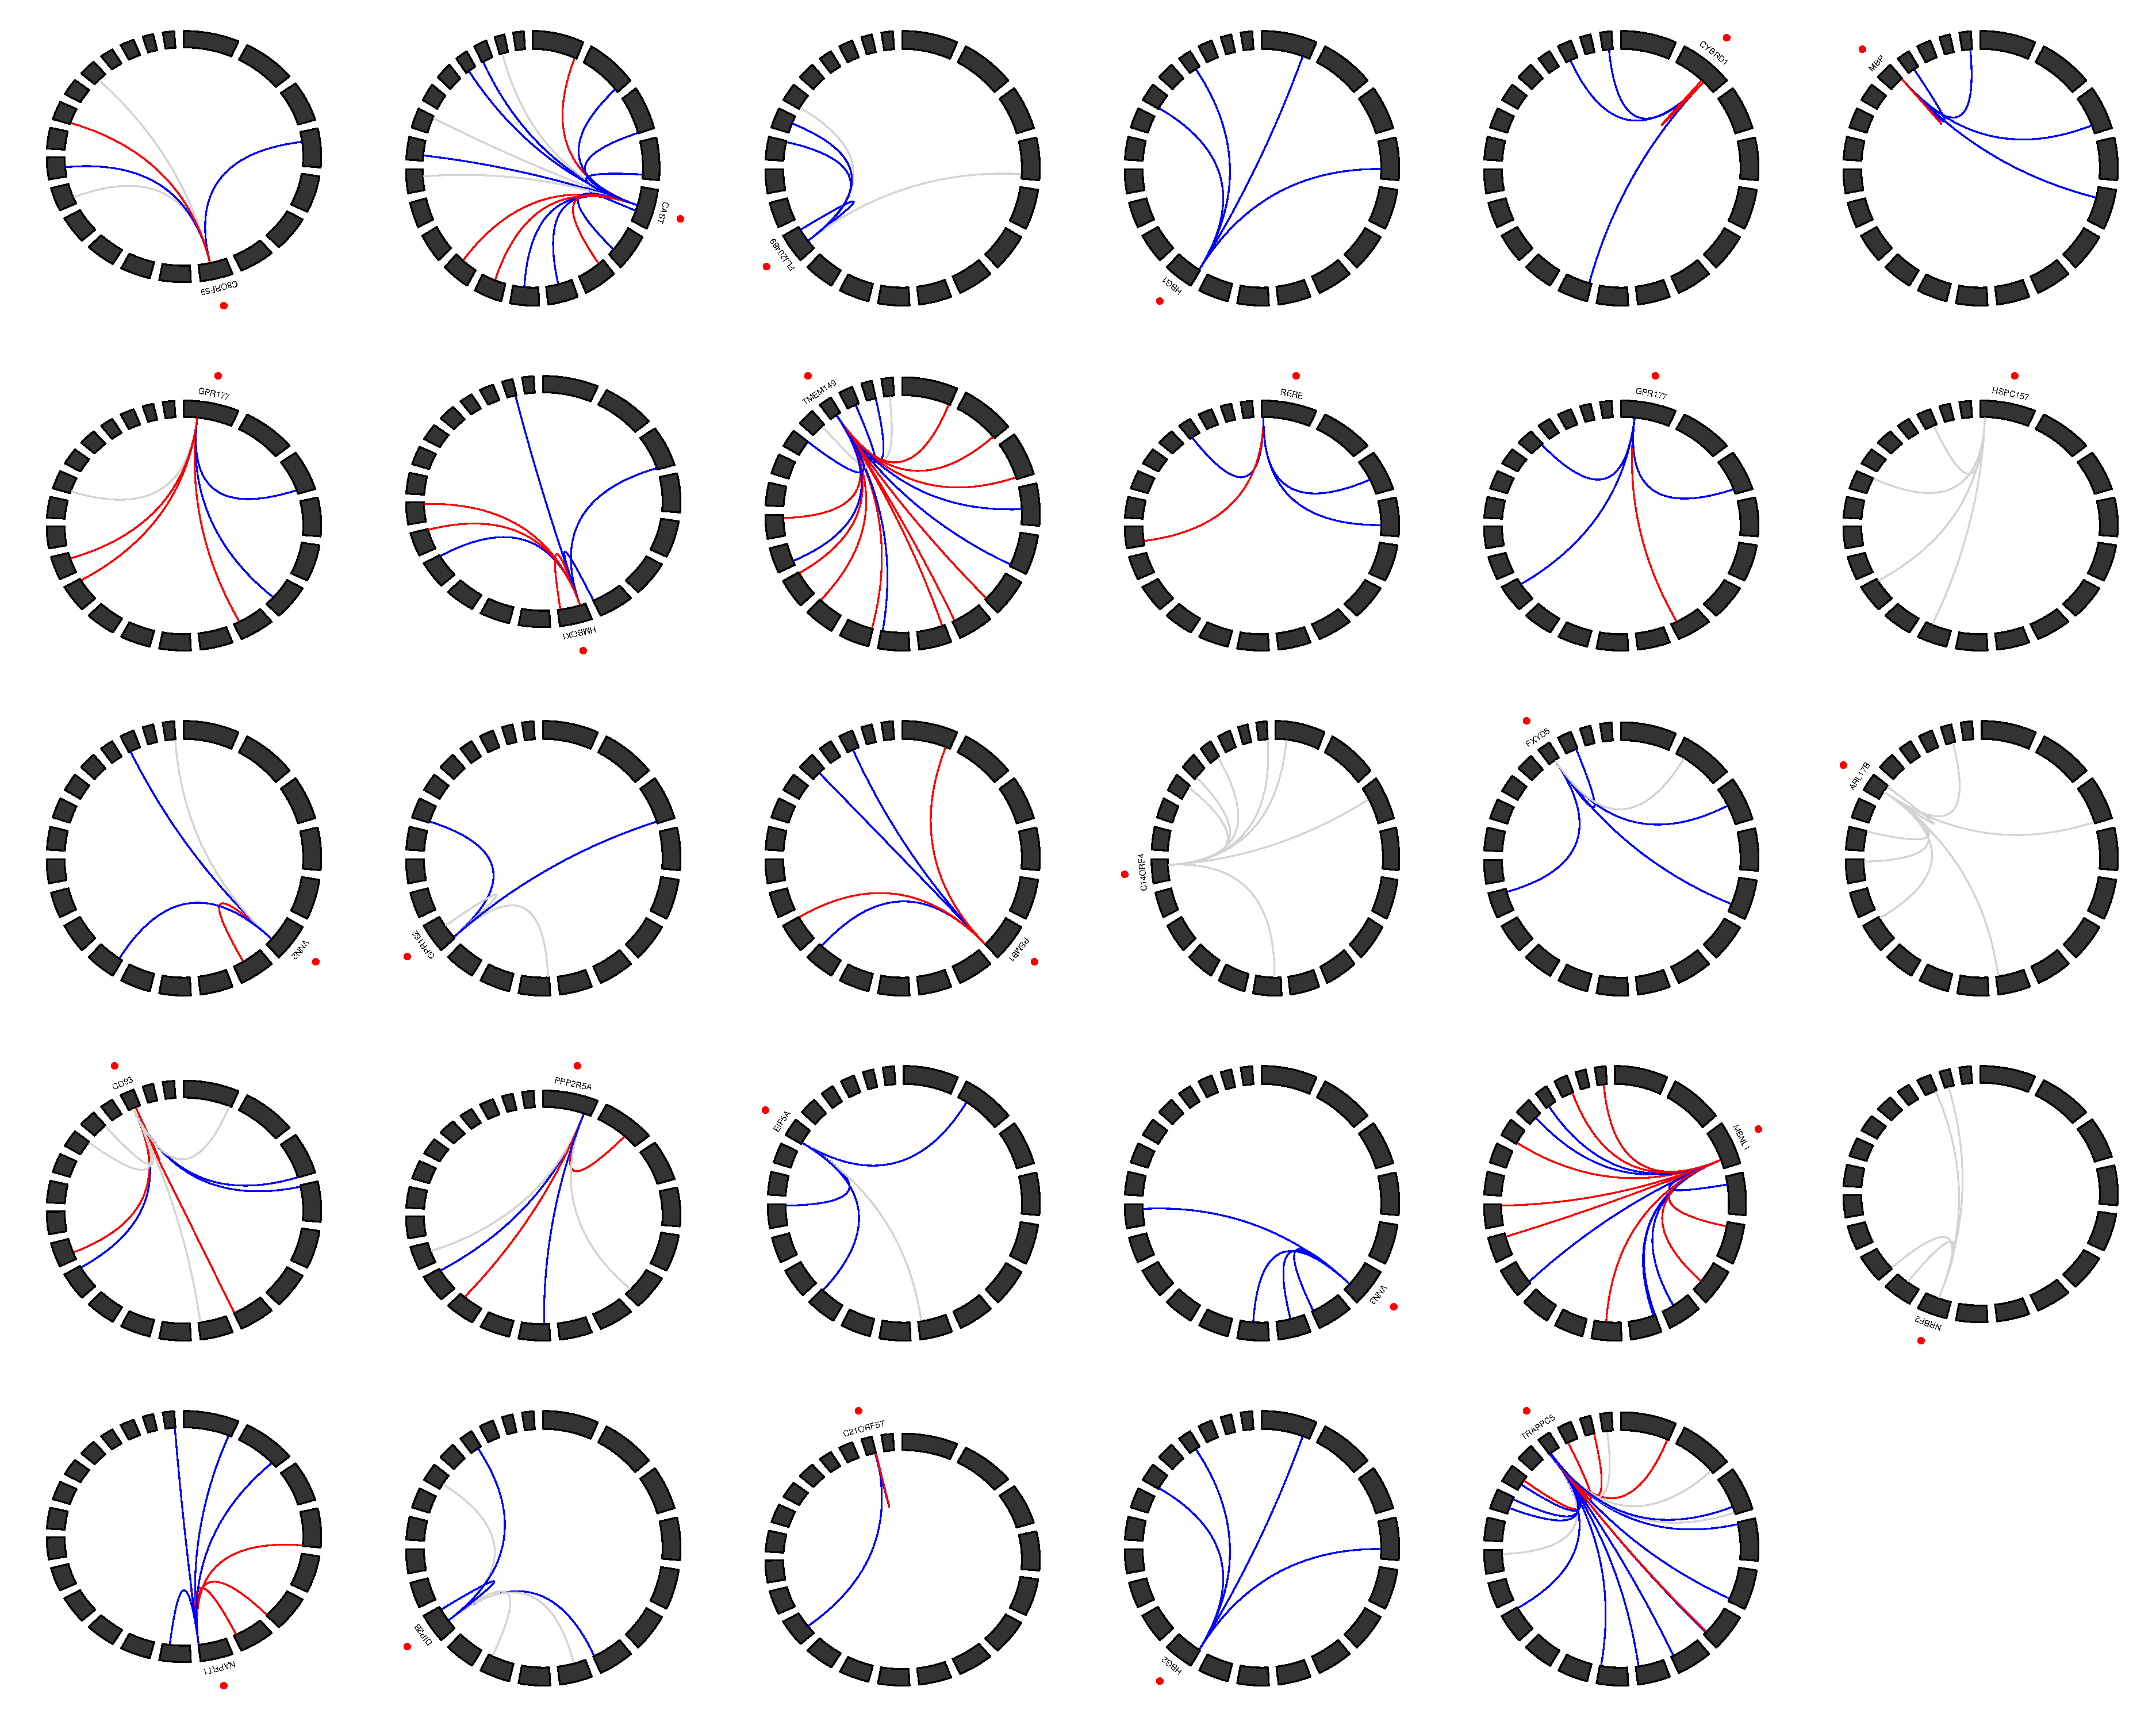
\includegraphics[width=5in]{circles_replication2}
	\caption{\textbf{Gene expression traits with four or more genetic interactions} Circle plots represent the genomic positions for SNPs (linking lines) and expression probes (red points). Chromosomes are represented by black blocks and ordered from 1 to 22 clockwise, starting from the top. Grey lines represent no evidence for replication, blue lines denote replication in at least one dataset, and red lines denote replication in two datasets. Most interactions are characterised as being \emph{cis}-\emph{trans} to the expression probe.}
	\label{fig:circleplots}
\end{figure}
\clearpage

\begin{figure}
	\centering
	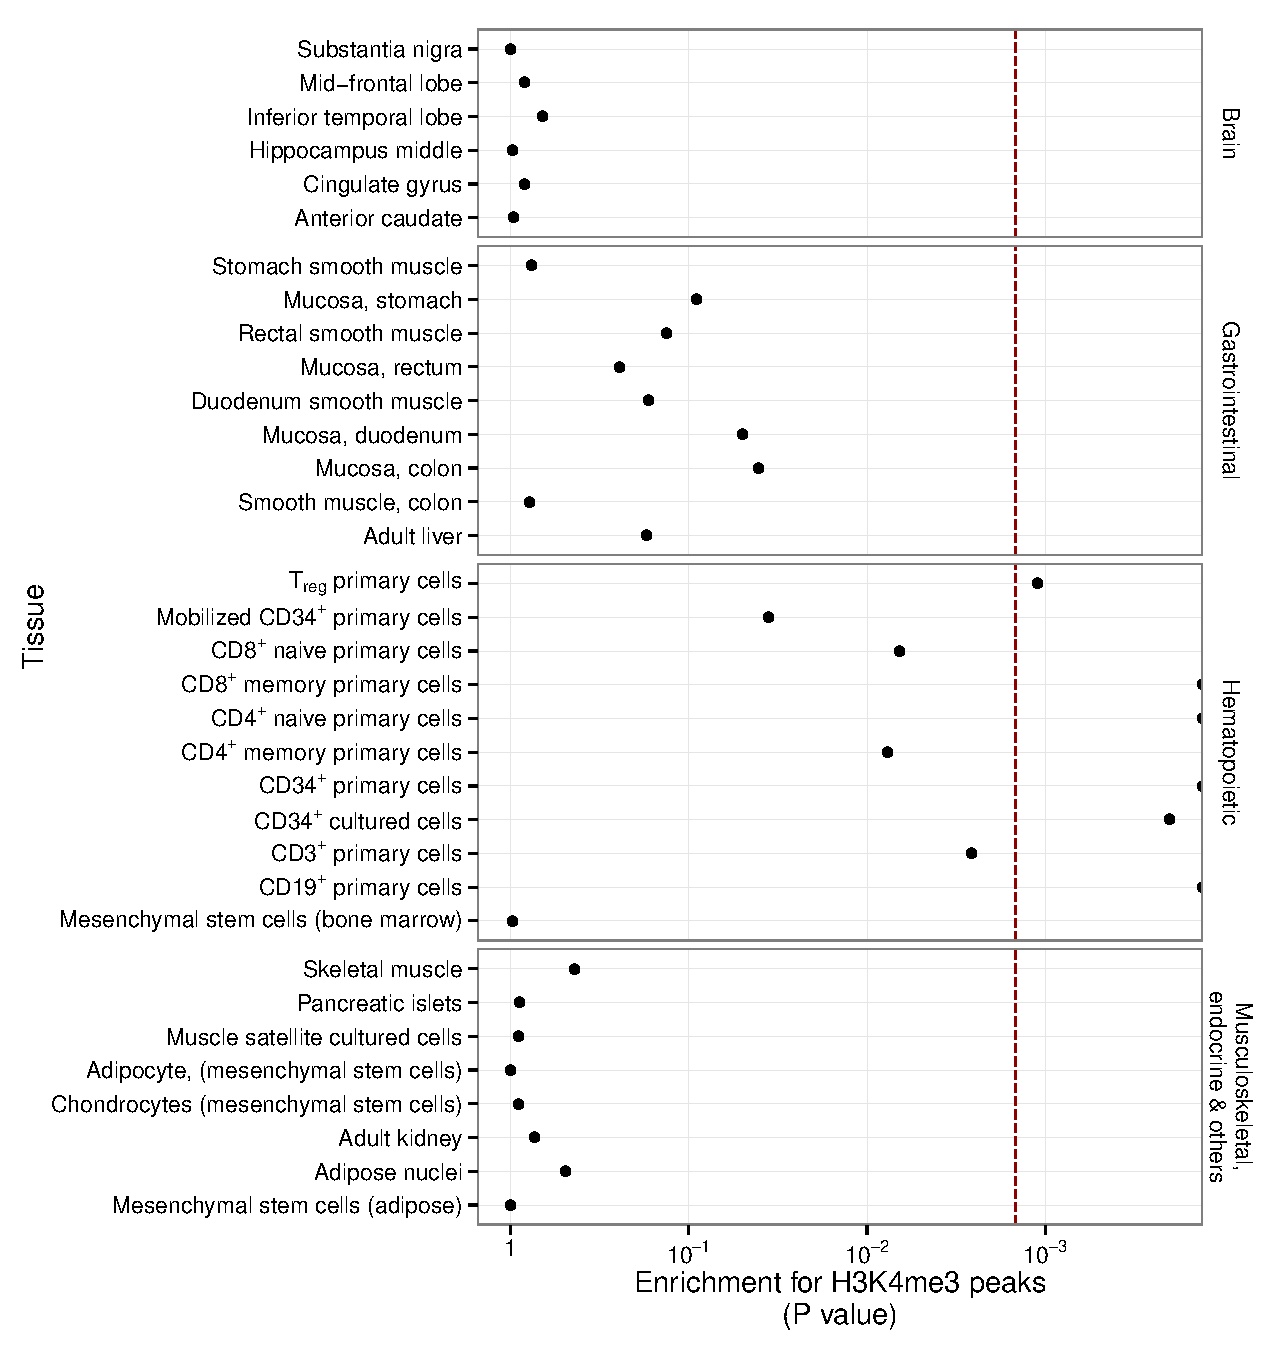
\includegraphics[width=5in]{cis_h3k4me3}
	\caption{\textbf{Tissue specific enrichment of SNPs in transcriptionally active regions} The locations of transcriptional activity can be predicted by chromatin marks, assayed by H3K4me3. Here we show that there is }
	\label{fig:cish3k4me3}
\end{figure}

\begin{figure}
	\centering
	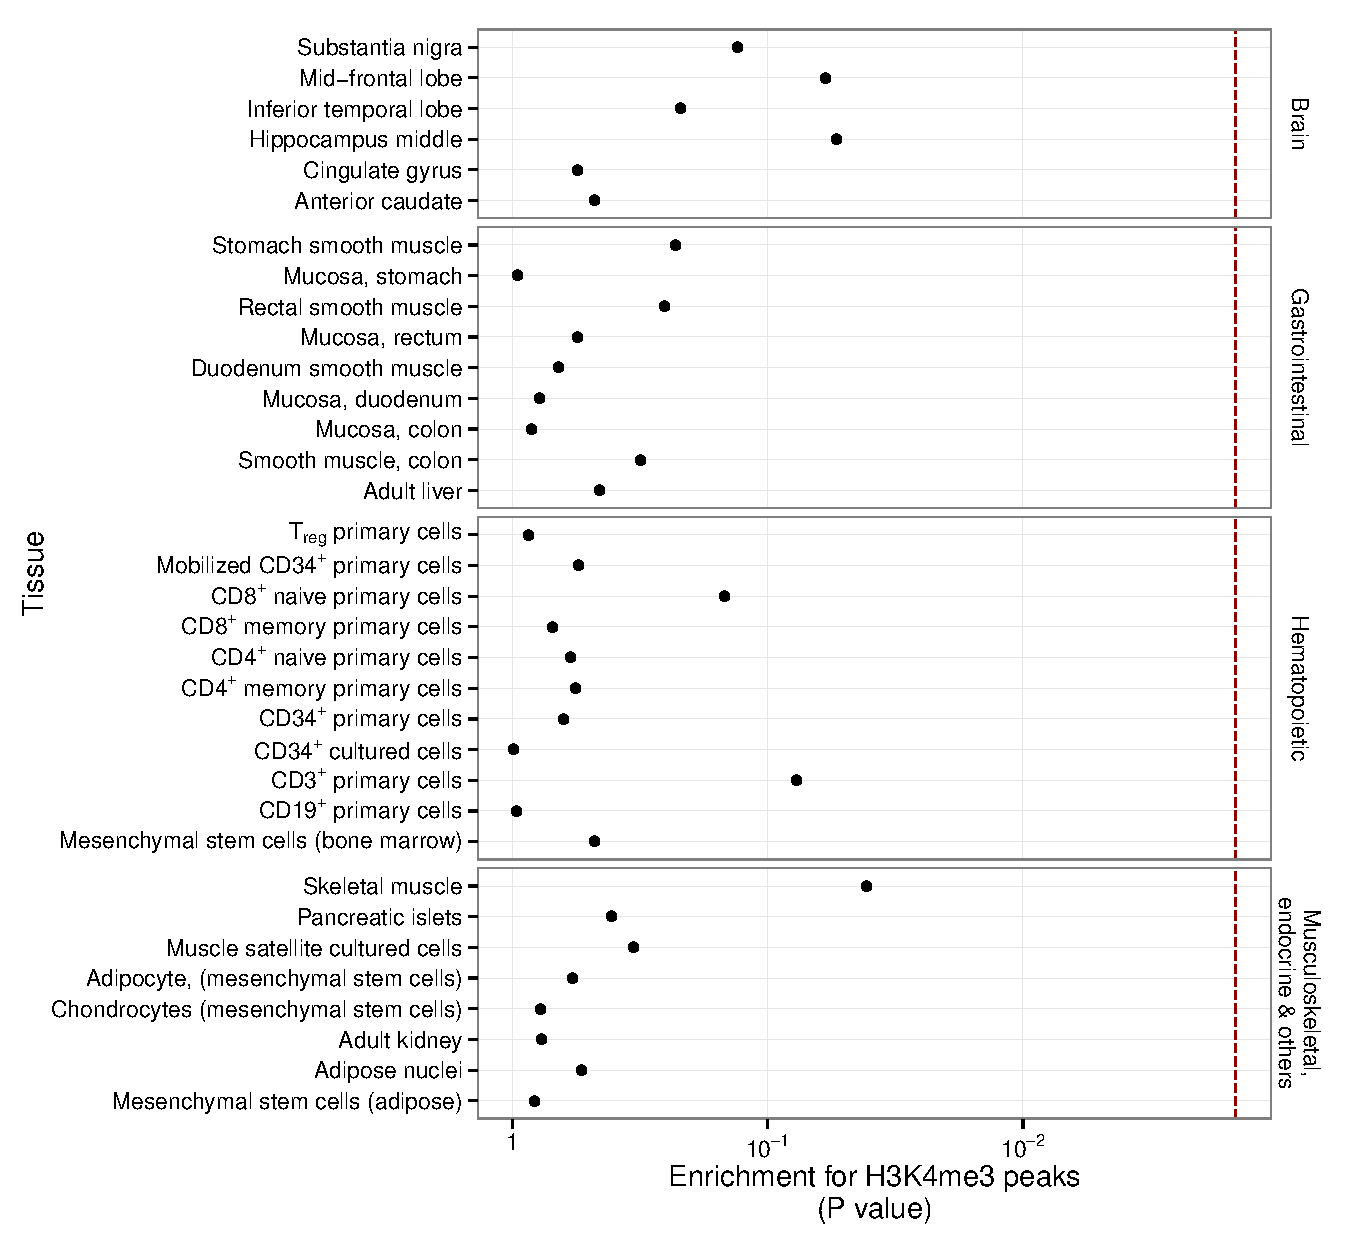
\includegraphics[width=5in]{trans_h3k4me3}
	\caption{\textbf{Tissue specific enrichment of SNPs in transcriptionally active regions} The locations of transcriptional activity can be predicted by chromatin marks, assayed by H3K4me3. Here we show that there is }
	\label{fig:transh3k4me3}
\end{figure}
\clearpage

\begin{figure}
	\centering
	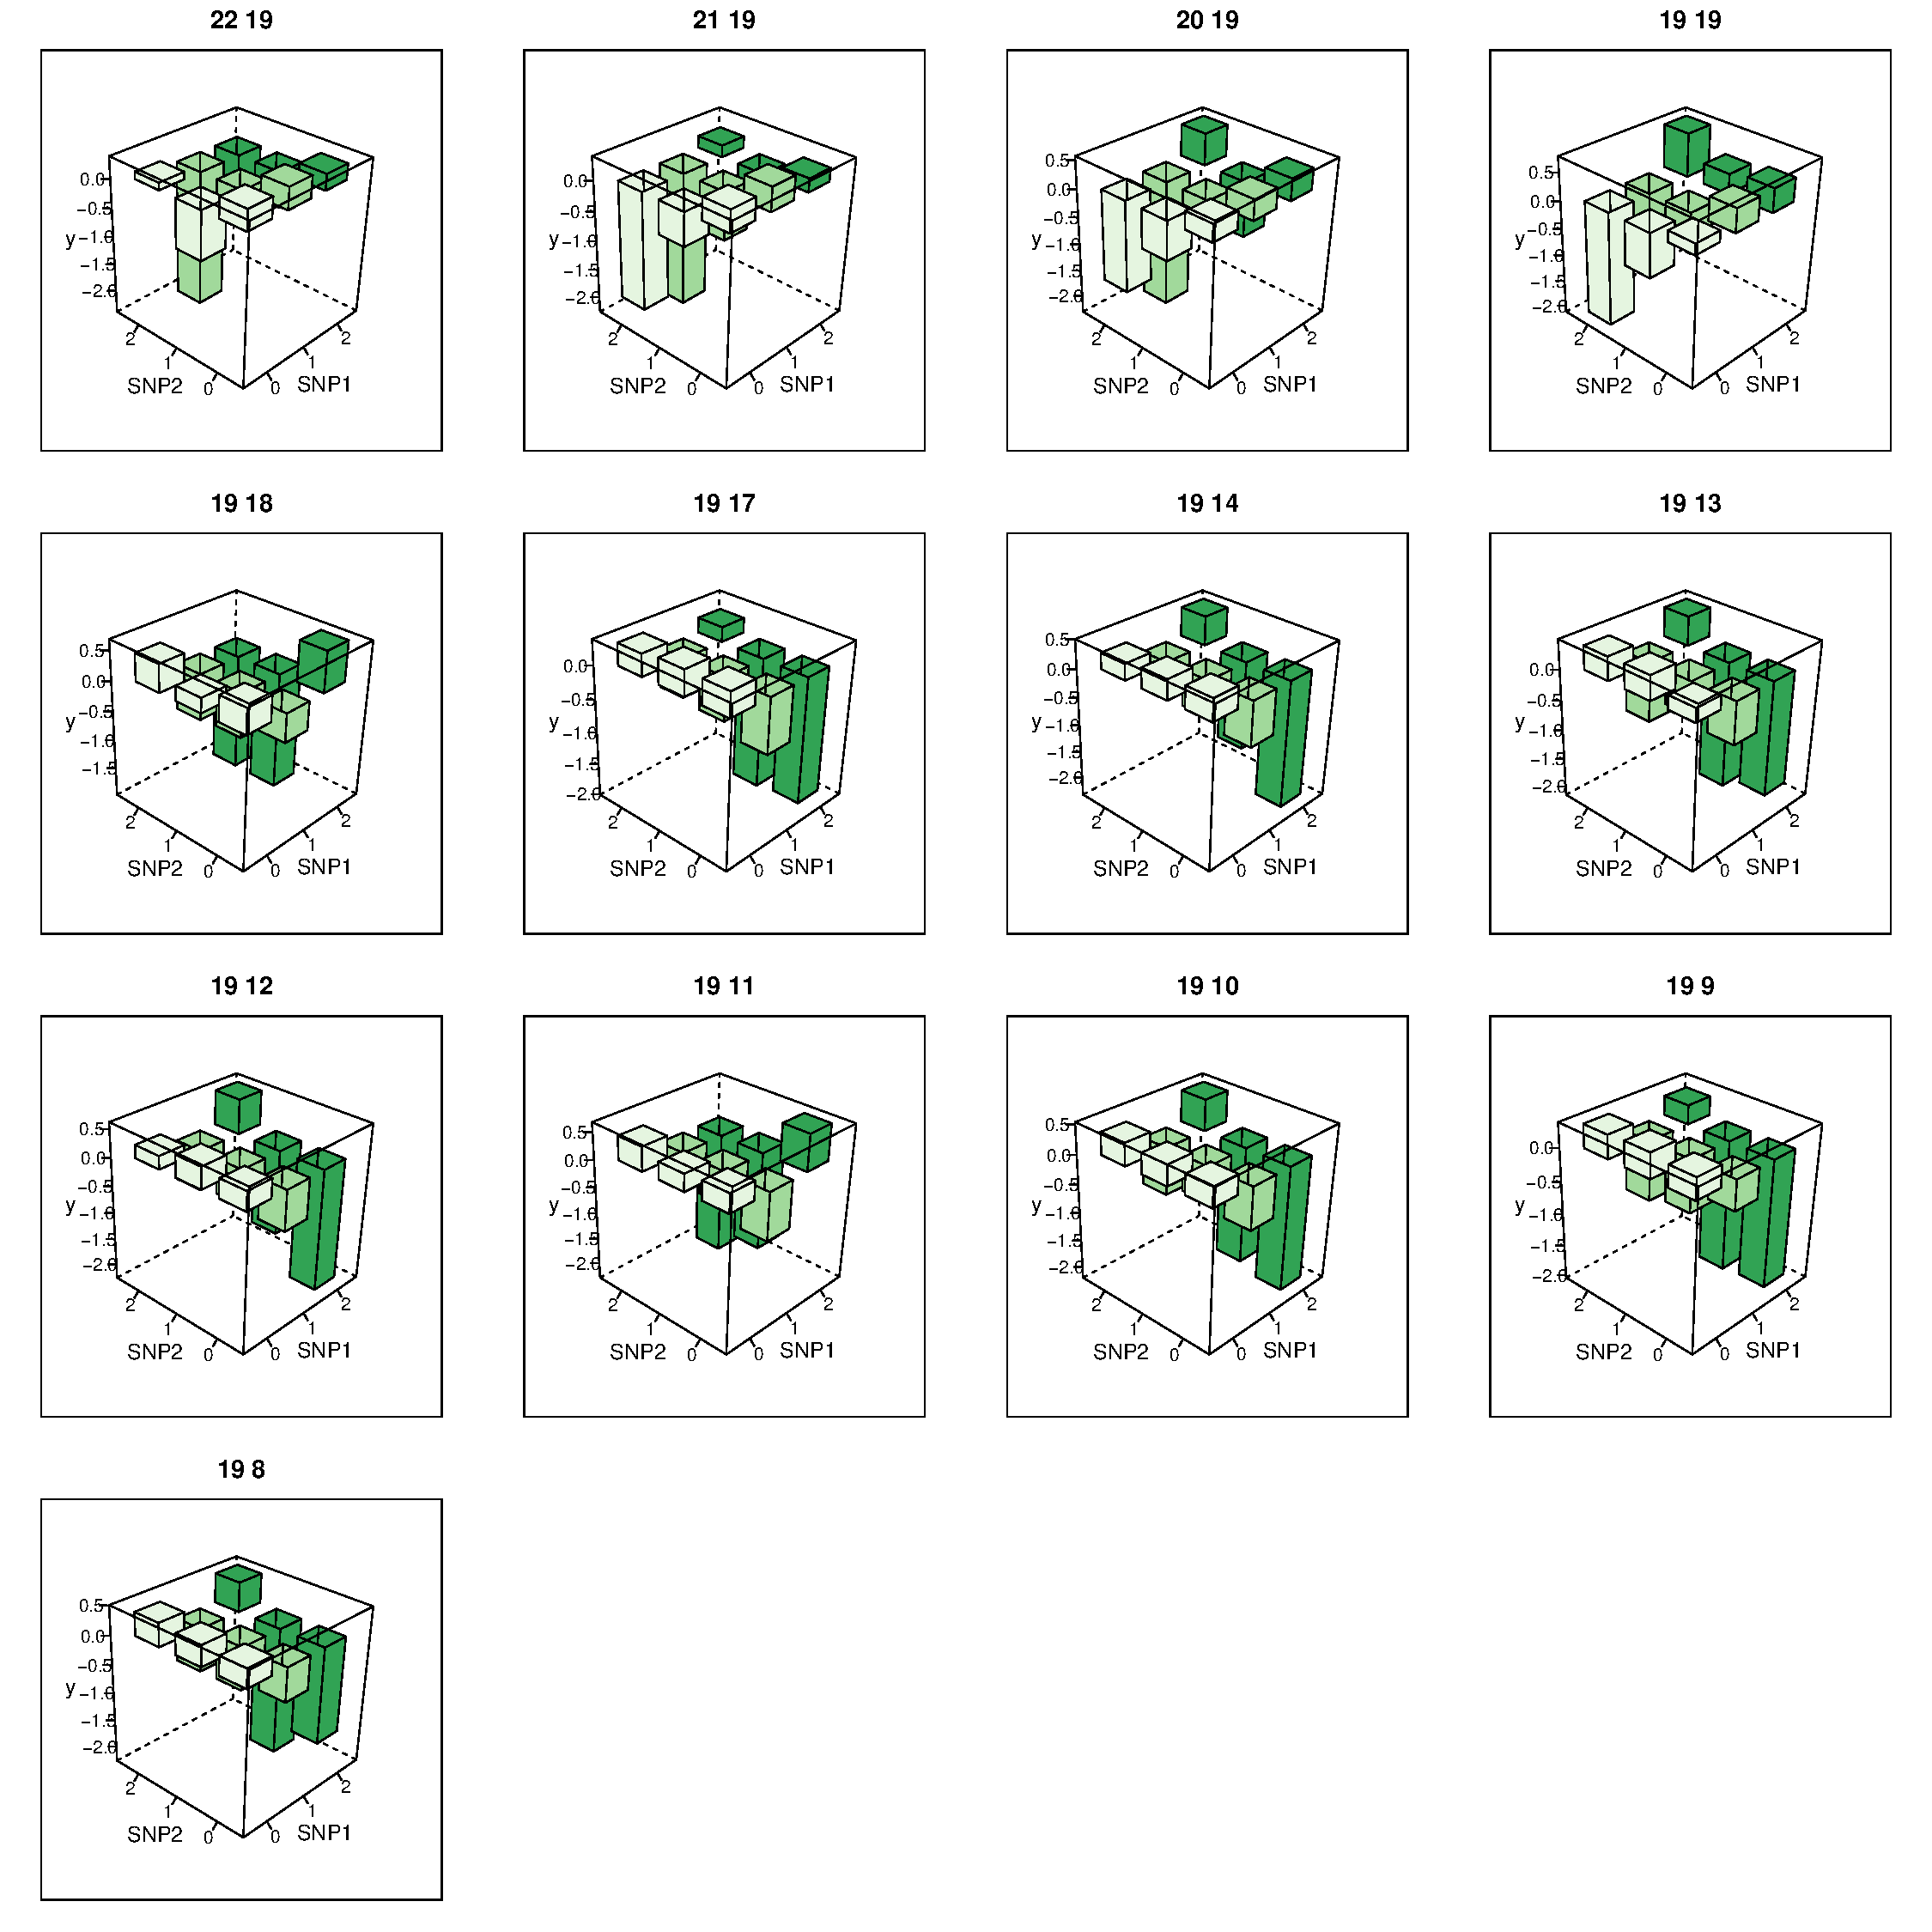
\includegraphics[width=5in]{MBNL1}
	\caption{\textbf{Genotype-phenotype maps for 14 interactions controlling MBNL1} Each bar represents the mean phenotypic value for individuals in that genotype class. The rs13069559 SNP typically has a \emph{cis}-additive decreasing effect on the expression of MBNL1, but in many of these interactions the \emph{cis} effect is masked when the \emph{trans} SNP is homozygous.}
	\label{fig:mbnl13d}
\end{figure}
\clearpage

\begin{figure}
	\centering
	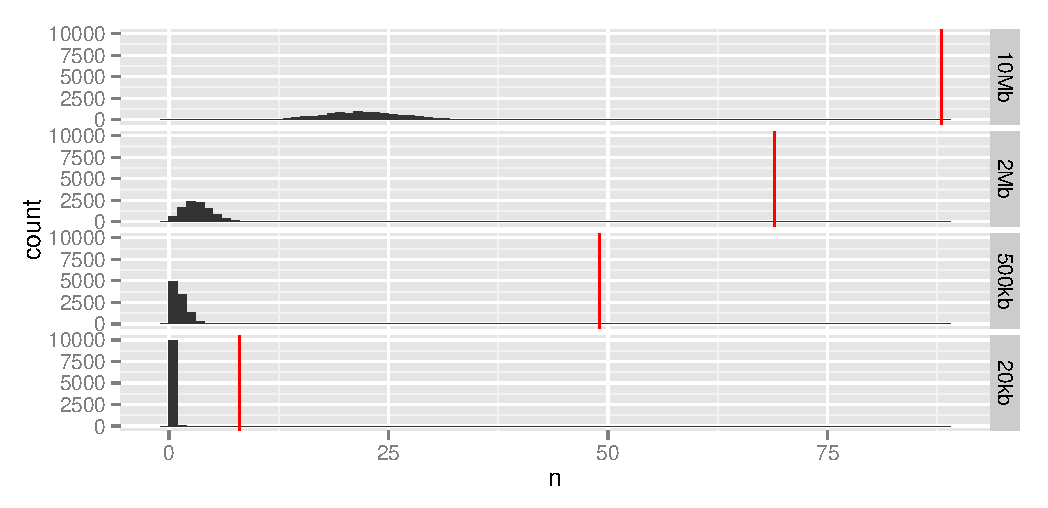
\includegraphics[width=5in]{chromosome_interactions}
	\caption{\textbf{Number of overlaps between chromosome interactions and epistatic interactions} Interacting chromosome regions may be a possible mechanism underlying epistatic interactions. The number of epistatic interactions within 20kb, 500kb, 2Mb and 10Mb of known chromosome interacting regions are shown by red vertical lines. The histograms represent the null distribution based on random sampling of 10000 datasets for each window size.}
	\label{fig:chromosomeinteractions}
\end{figure}
\clearpage

\begin{figure}
	\centering
	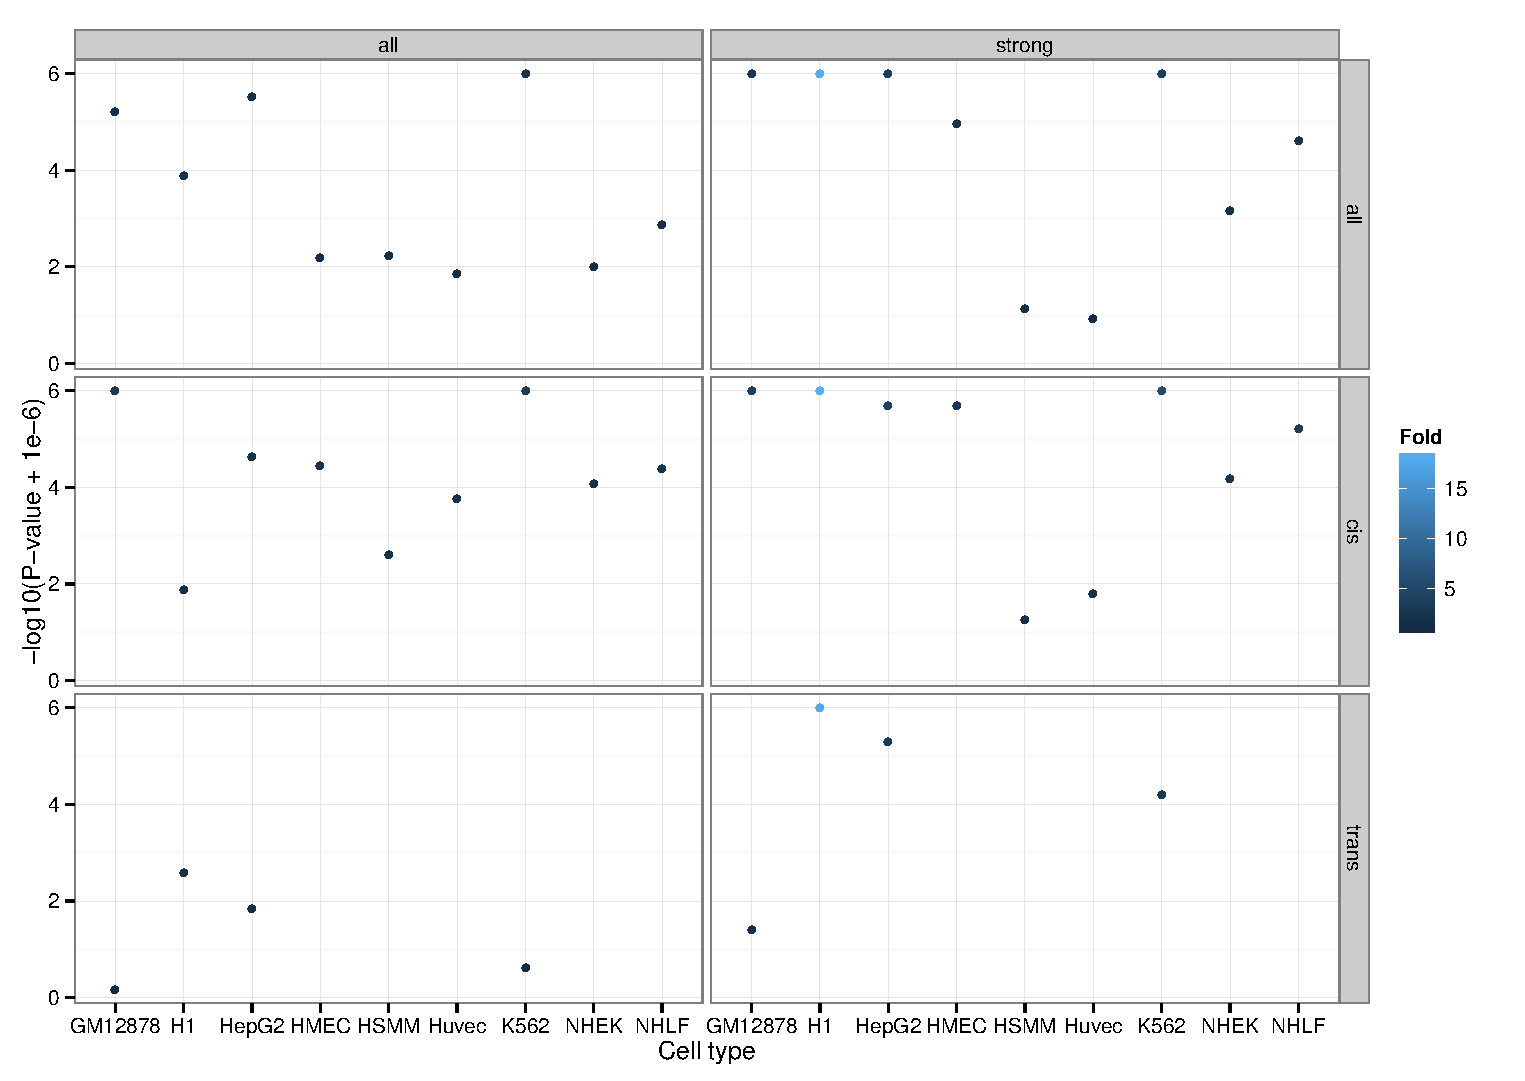
\includegraphics[width=5in]{enhancers}
	\caption{\textbf{There is enrichment for enhancer sequences for \emph{cis} and \emph{trans} SNPs}}
	\label{fig:enhancers}
\end{figure}

\begin{figure}
	\centering
	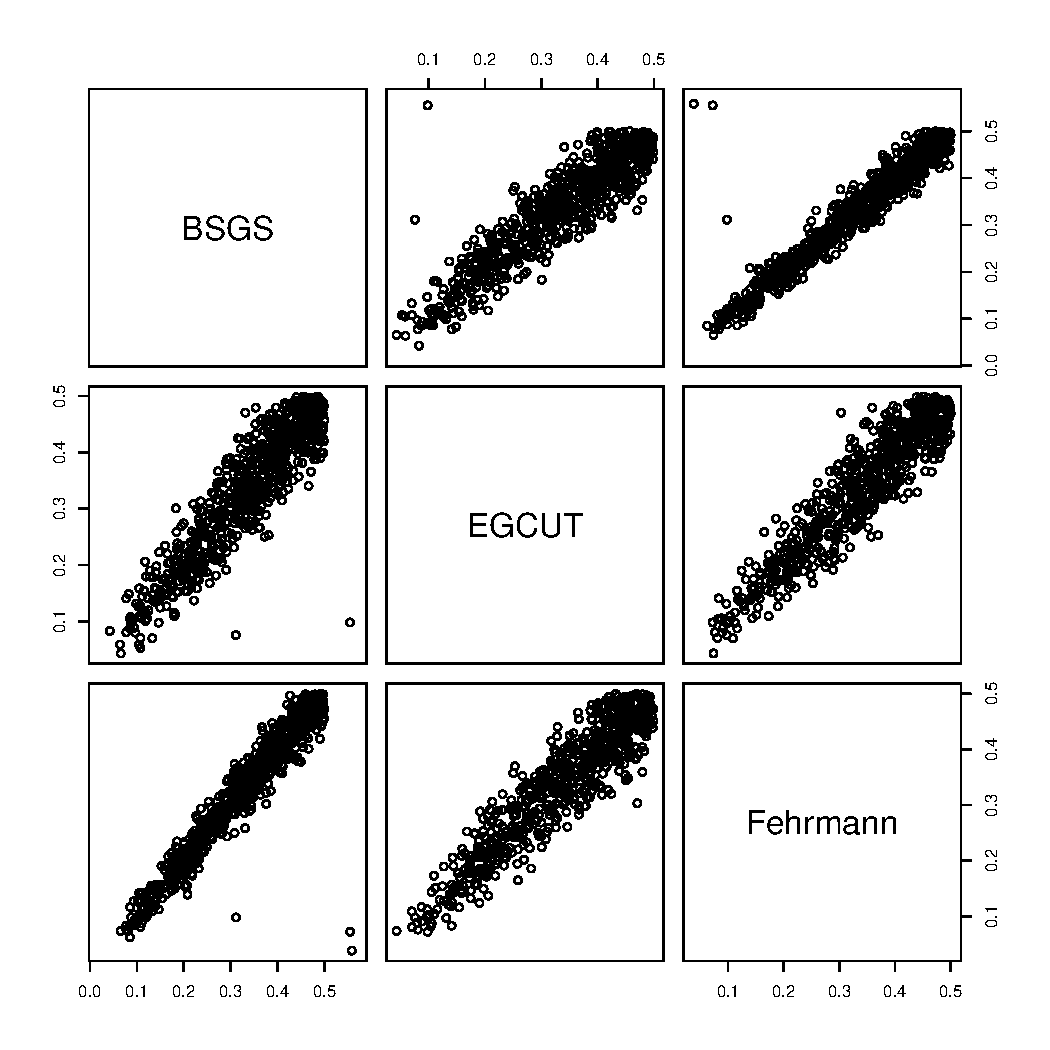
\includegraphics[width=5in]{alleleFreq}
	\caption{\textbf{Comparison of allele frequencies for 781 SNPs involved in genetic interactions across independent populations} Outliers were removed from the analysis as part of the filtering stage during replication.}
	\label{fig:allelefreq}
\end{figure}




\clearpage
\section{References}
\bibliography{refs}

\end{document}